\chapter{The \chips R\&D Project}
\label{chap:chips}

%%%%%%%%%%%%%%%%%%%%%%%%%%%%%%%%%%%%%%%%%%%%%%%%%%%%%%%%%%%%%%%%%%%%%%%%%%%%%%%%%%%%%%%%%%%%%%%%%%
%                                              PLAN                                              %
%%%%%%%%%%%%%%%%%%%%%%%%%%%%%%%%%%%%%%%%%%%%%%%%%%%%%%%%%%%%%%%%%%%%%%%%%%%%%%%%%%%%%%%%%%%%%%%%%%
\begin{comment}
TODO: Write the story of the chips chapter

TODO: Write the chips chapter section outline

TODO: Add all the sections below

TODO: Read through all CHIPS related papers and make general notes in appropriate subsections
\end{comment}

%%%%%%%%%%%%%%%%%%%%%%%%%%%%%%%%%%%%%%%%%%%%%%%%%%%%%%%%%%%%%%%%%%%%%%%%%%%%%%%%%%%%%%%%%%%%%%%%%%
%                                          INTRODUCTION                                          %
%%%%%%%%%%%%%%%%%%%%%%%%%%%%%%%%%%%%%%%%%%%%%%%%%%%%%%%%%%%%%%%%%%%%%%%%%%%%%%%%%%%%%%%%%%%%%%%%%%
\section{Introduction}
\label{sec:chips_intro}
\begin{comment}
- General overview of why a large, cheap detector like CHIPS is needed
- Brief overview of what CHIPS could add to physics, what it can detect etc...
- general non-detailed description of the general principles behind CHIPS
- CHIPS a large, yet cost-effective water chereknov detector concept, to initially run in the
Numi beam line.
- Will be deployed in a flooded mine pit, which removes the necessity and expense of a substantial
external structure to support the large detector mass.
- Will be initially deployed into the Wentworth Pit 2W in northen minnesota, which is 7 mrad
off-axis of the numi beam.
- Also deep enough to allow for ~50m of everburden of water to reduce the cosmic background.
- Can easily be deployed in the LBNF beam once operational.
- Can help to constrain delta-cp by measuring electron neutrino appearance.
- Not at the ideal location (baseline) to measure the mass hierarchy in the Numi beam.
- Physics capabilities have been studied using GLoBES, should ask Tom for a nice plot and brief
description of how it all works.
- Calculations indicate there will be 3.7 nutau CC interactions per kton per year. Leading to
~0.35 additional background effects per kton per year once selections are applied.
- Wentworth 2W is a disused surface iron pit (taconite ore) owned by Cliffs natural resources.
- Has advantages of having the infastrucutre in place for heavy industry, such as power and roads.
- The main Polymet mining building is less than a mile from the deployment site which was used as
a laboratory environment for building detector compoenents on site.
- located at a latitude of 47.58N and longitude of 92.13W. It is 7 mrad off the centralaxis of the
NuMI beam at a baseline of 712 km
- Water is drained from the pit in the spring to ensure it does not overflow during the summer
rainy season.
- Therefore, fluctutationsof +-3m are expected over the course of a year.
- Need to include the expected cosmic ray plots
DIAGRAM: expected cosmic rate at different height plot
- Instead of deploying very large single detectors which would be impractical, you can deploy
multiple independent cylindrical units.
- The detector height is then constrained by the depth of the water and the cosmic overburden
requirements.
- The chips-5 detector is the first of these units, at 25m in diameter and 12m tall.
- This leads to a fiducial volume of ~5kton
- A lighttight liner a polymer membrance is used to seperate the clean detector water from the
external pit water and isolate the detector volume.
- CHIPS uses high quantum efficiency PMTs from Hamamatsu
REF: Get hamamatsu PMT reference
INFO: detector module
- Dimensions
- Inner surface area
- PMT diameter
- photocathode coverage in different regions
- No of PMTs
- overburden
- CR muon rate
- In-spill CR occupancy
- CR event dead time
- Veto dimensions
- Veto num PMTs
- veto photocathode coverage
- veto pmt diameter

- Give full description of how each plane is constructed, how they are attached to the detector.
- Full description of the detector structure
- Full description of deployment/construction procedure
- Description of how the liner is built etc
- Though remarkably clear the Wentworth pit water is not clean enough for the detector volume
where we require ~30m attenuation length.
- This detector will act as a proff of concept that the R&D has been a success and the provide
possible improvements for future iterations.
- CHIPS will not initially have a near detector, however the use of NOVA one is possible if
required, but not important for now.
- You would really need a water cherenkov near detector, so it as simiar as possible as the far
detector.
- This allows the same event reco and PID minimising systematic uncertainties in the predicted
background at the far detector.
- Is prefered as it has the same neutrino interaction traget (water) ensuring efficiencies are
similar in both detector.
- However, it should be noted that a water cherenkov detector has never been proven in high
intensity environmenets such as the Numi beam (WTF is t2k then)
- For calibration "flashers" are built into the detector to allow for known location light
generation to calibrate final PMT positions and time resolutuions.
- We take full advantage of the MINOS, NOVA extensive simulations of the Numi beam for use in
CHIPS.
DIAGRAM: Alongside numi flux have numu distribution at chips with and without oscillations, can
just take from letter of intent if required.

Hyper-k letter of intent~\cite{abe2011}
Dune CDR~\cite{acciarri2016}
\end{comment}

%%%%%%%%%%%%%%%%%%%%%%%%%%%%%%%%%%%%%%%%%%%%%%%%%%%%%%%%%%%%%%%%%%%%%%%%%%%%%%%%%%%%%%%%%%%%%%%%%%
%                                    NEUTRINO EVENTS AT CHIPS                                    %
%%%%%%%%%%%%%%%%%%%%%%%%%%%%%%%%%%%%%%%%%%%%%%%%%%%%%%%%%%%%%%%%%%%%%%%%%%%%%%%%%%%%%%%%%%%%%%%%%%
\section{Events for the CHIPS detector}
\label{sec:chips_events}
\begin{comment}
- First how beam water Cherenkov detect events
- Describe the Numi beam
- An aside on the off-axis effect
- Describe the Cherenkov effect
- Describe the flux and expected cross-sections / types of event
- Give the expected number of events that CHIPS should see
- An aside on GENIE which we used for event generation
- Describe all the possible interactions that can be observed in CHIPS
- What are the classic difficulties with water Cherenkov detectors
- Brief description of how PMTs detect the cherenkov light
- CHIPS detector simulation
- Example plots of events for different signature types of events...
- We always need to consider the two main signal channels muon dissapearance and electon
appearance, and their main backgrounds
NC 1pi+- and 1pi0 respectively.
\end{comment}

EQUATION: Off-axis effect equations
EQUATION: Cherenkov effect equation

- The CHIPS-M detector and conclusions
- The CHIPS-10 detector
- General structure, how it all holds together
- How it is deployed/extended
- How it detects the Cherenkov light with PMTs arranged in planes
- How the construction went
- Current status and future plans
- The tau neutrino component is negligible and not predicted by the simulation

\begin{figure} % CHIPS SUNRISE DIAGRAM %%%%%%%%%%%%%%%%%%%%%%%%%%%%%%%%%%%%%%%%%%%%%%%%%%%%%%%%%%%
    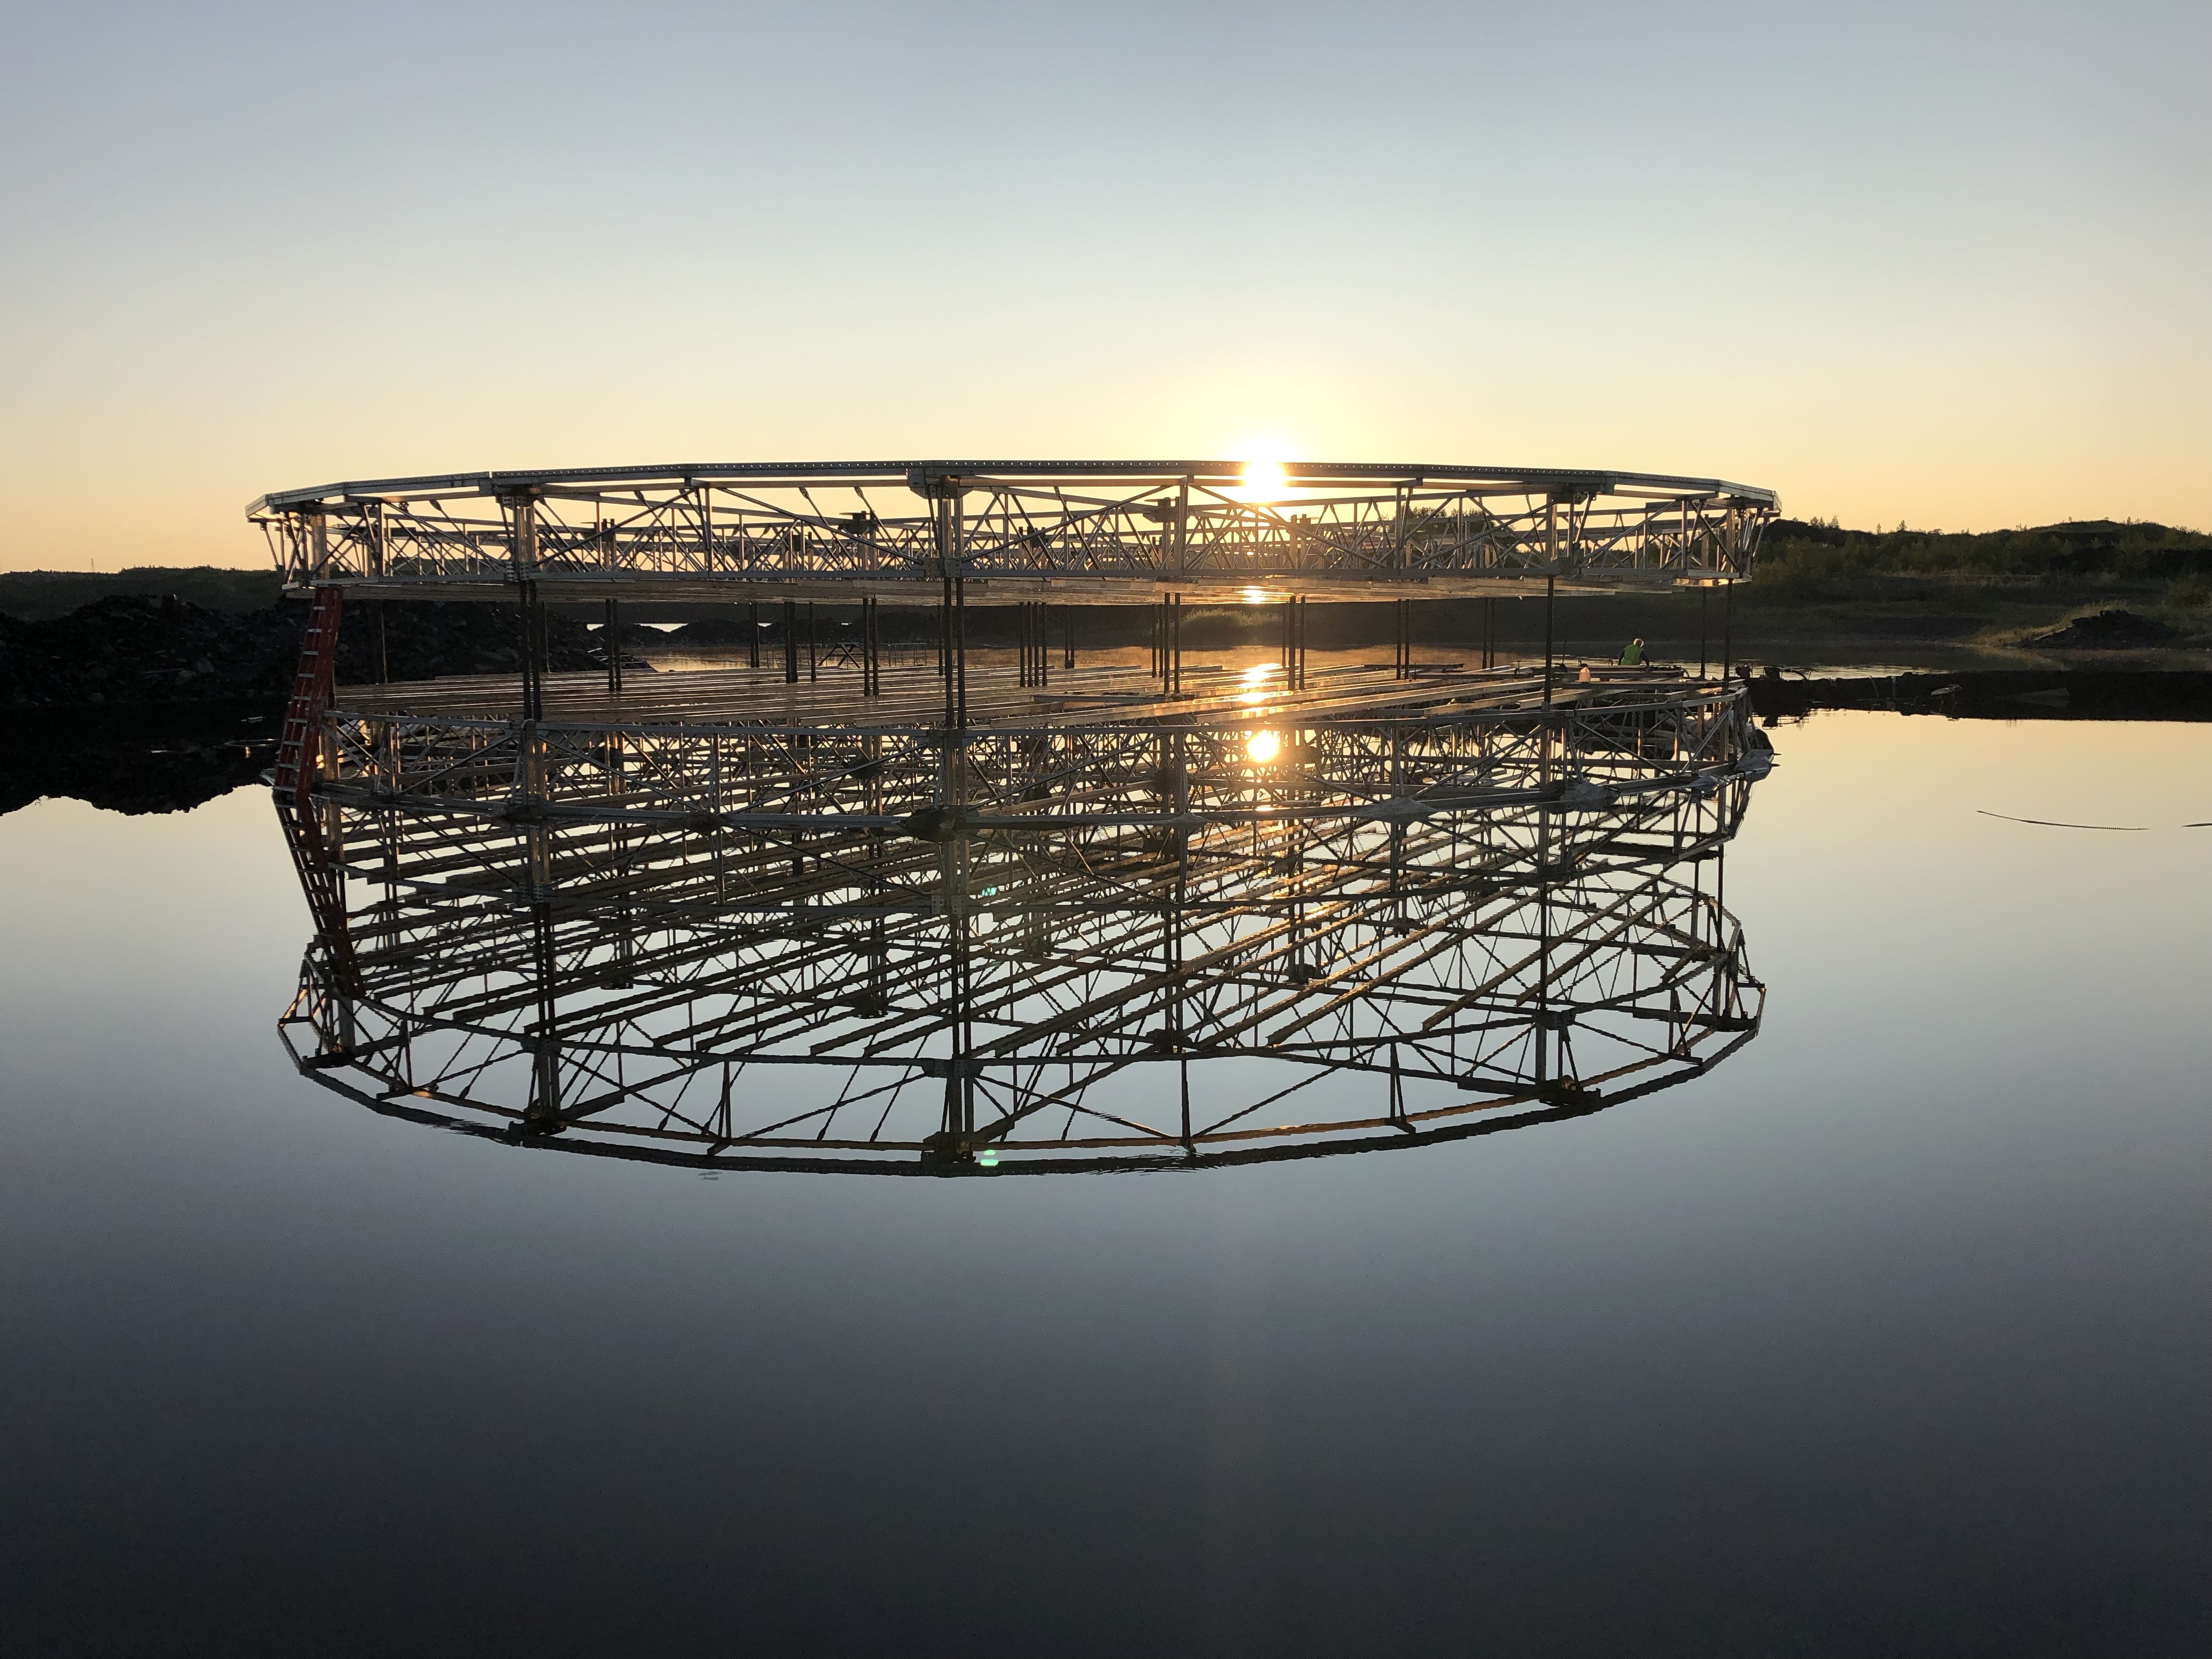
\includegraphics[width=0.8\textwidth]{diagrams/5-chips/sunrise.jpeg}
    \caption[Sunrise over the \chips detector.]
    {Sunrise over the \chips detector structure. The perfectly calm pit water
        produces the mirror effect.}
    \label{fig:sunrise}
\end{figure} %%%%%%%%%%%%%%%%%%%%%%%%%%%%%%%%%%%%%%%%%%%%%%%%%%%%%%%%%%%%%%%%%%%%%%%%%%%%%%%%%%%%%

\begin{figure} % CHIPS FROM THE SKY DIAGRAM %%%%%%%%%%%%%%%%%%%%%%%%%%%%%%%%%%%%%%%%%%%%%%%%%%%%%%
    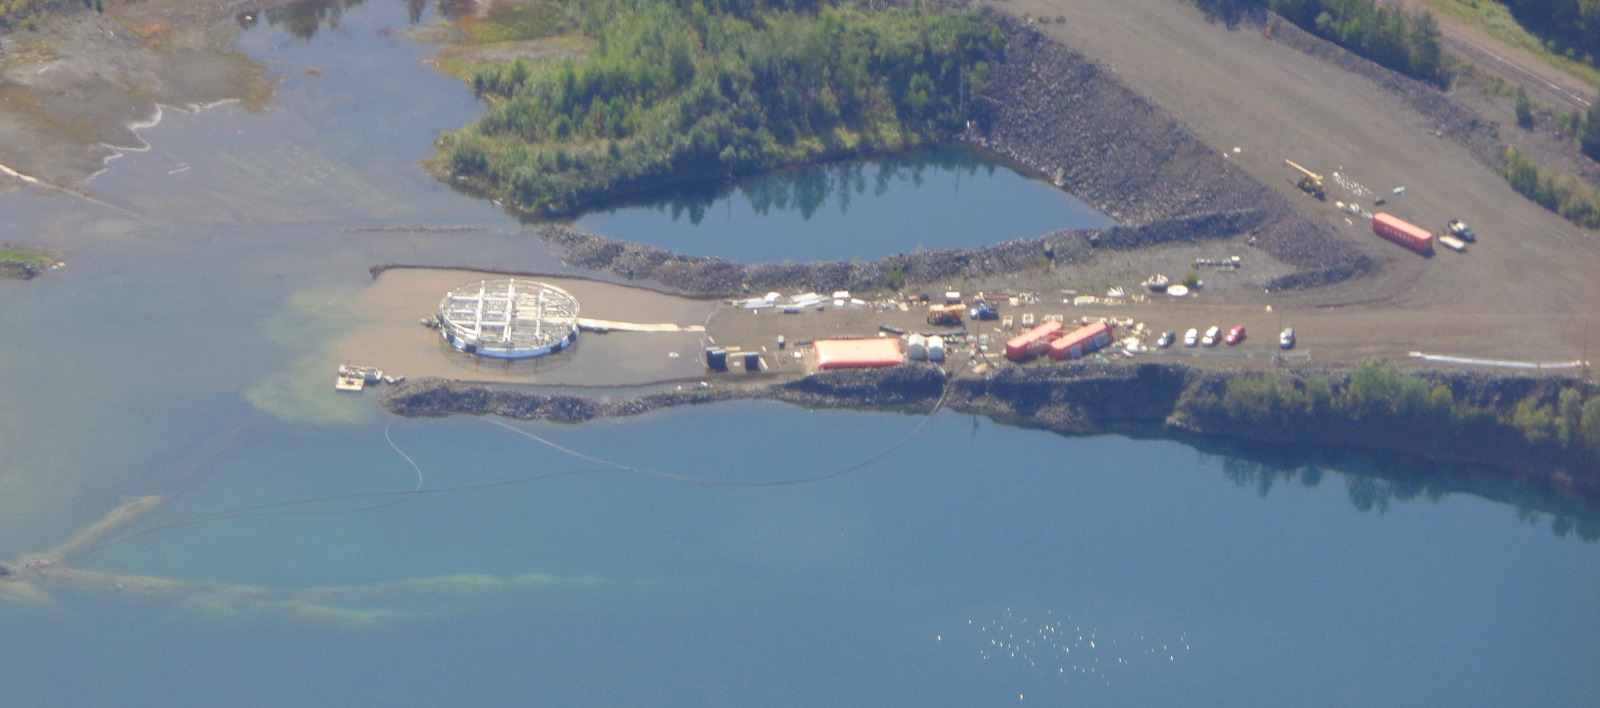
\includegraphics[width=0.8\textwidth]{diagrams/5-chips/from_the_sky.jpg}
    \caption[Picture of the \chips detector from the air.]
    {Picture of the \chips detector taken from an airplane. The Wentworth 2W pit is in the lower
        half of the image, with the half built detector, huts and construction containers
        visable.}
    \label{fig:from_the_sky}
\end{figure} %%%%%%%%%%%%%%%%%%%%%%%%%%%%%%%%%%%%%%%%%%%%%%%%%%%%%%%%%%%%%%%%%%%%%%%%%%%%%%%%%%%%%

\begin{figure} % PIT DIAGRAM %%%%%%%%%%%%%%%%%%%%%%%%%%%%%%%%%%%%%%%%%%%%%%%%%%%%%%%%%%%%%%%%%%%%%
    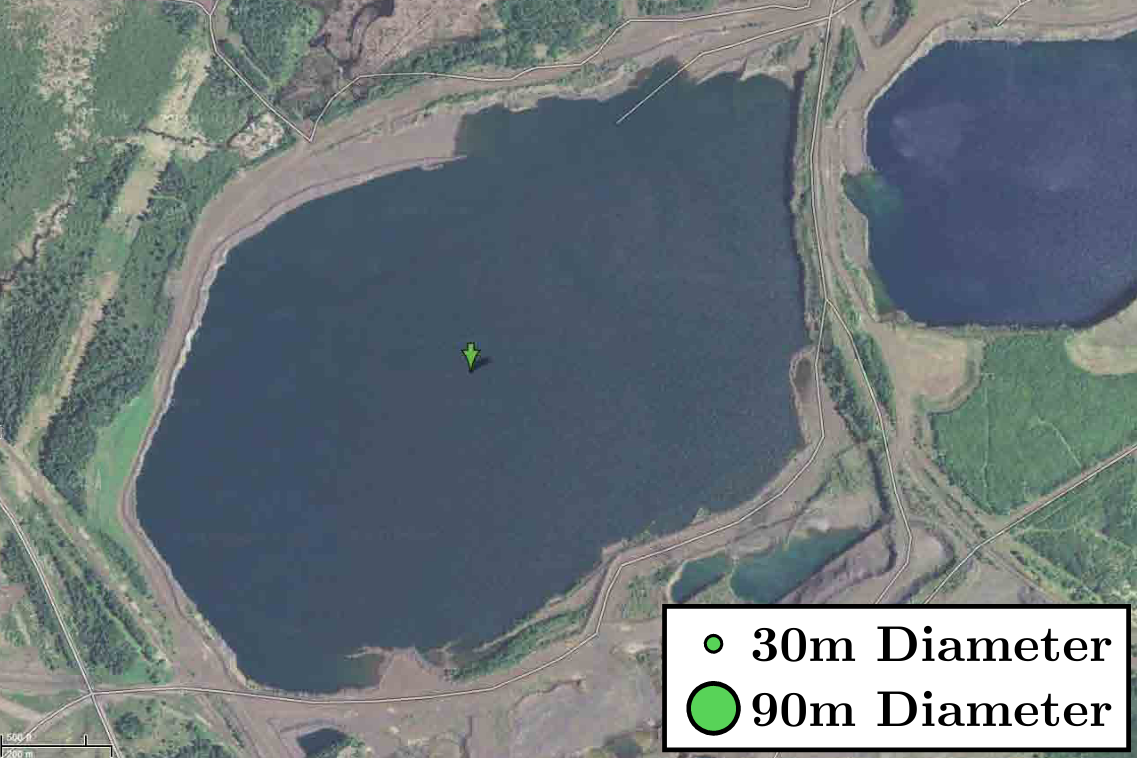
\includegraphics[width=0.8\textwidth]{diagrams/5-chips/location.png}
    \caption[Satellite view of the Wentworth 2W mine pit.]
    {Satellite view of the Wentworth 2W mine pit in northern Minnesota.
        The size markers are shown for scale. Image taken from Ref.\cite{adamson2013}.}
    \label{fig:location}
\end{figure} %%%%%%%%%%%%%%%%%%%%%%%%%%%%%%%%%%%%%%%%%%%%%%%%%%%%%%%%%%%%%%%%%%%%%%%%%%%%%%%%%%%%%

\begin{figure} % PIT CONTOUR DIAGRAM %%%%%%%%%%%%%%%%%%%%%%%%%%%%%%%%%%%%%%%%%%%%%%%%%%%%%%%%%%%%%
    \includegraphics[width=0.8\textwidth]{diagrams/5-chips/contour_map.pdf}
    \caption[Topographic map of the Wentworth 2W mine pit.]
    {Topographic map of the Wentworth 2W mine pit. The contours are given in intervals of 5 feet,
        with the central areas of the pit having a depth of 50m. Image taken from
        Ref.\cite{adamson2013}.}
    \label{fig:contour_map}
\end{figure} %%%%%%%%%%%%%%%%%%%%%%%%%%%%%%%%%%%%%%%%%%%%%%%%%%%%%%%%%%%%%%%%%%%%%%%%%%%%%%%%%%%%%

\begin{figure} % CHIPS-M DIAGRAM %%%%%$$$%%%%%%%%%%%%%%%%%%%%%%%%%%%%%%%%%%%%%%%%%%%%%%%%%%%%%%%%%
    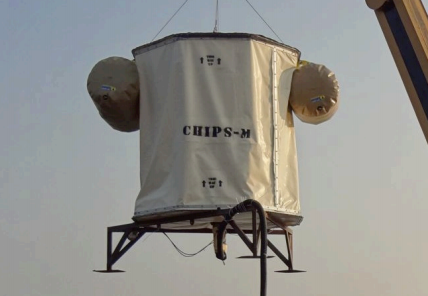
\includegraphics[width=0.8\textwidth]{diagrams/5-chips/chips_m.png}
    \caption[Picture of the \chipsm detector.]
    {Picture of the \chipsm detector just before deployment. The umbilical is visable, attached to
        the bottom endcap of the detector.}
    \label{fig:chips_m}
\end{figure} %%%%%%%%%%%%%%%%%%%%%%%%%%%%%%%%%%%%%%%%%%%%%%%%%%%%%%%%%%%%%%%%%%%%%%%%%%%%%%%%%%%%%

\begin{figure} % CHIPS RENDER 1 DIAGRAM %%%%%%%%%%%%%%%%%%%%%%%%%%%%%%%%%%%%%%%%%%%%%%%%%%%%%%%%%%
    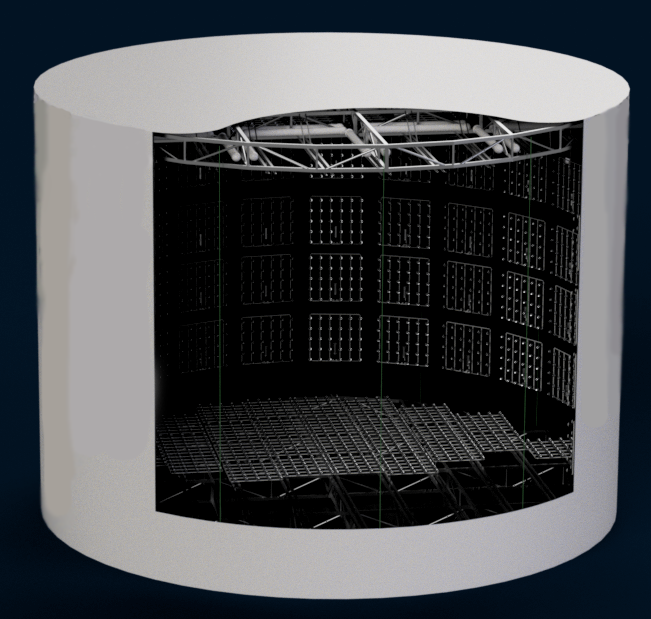
\includegraphics[width=0.8\textwidth]{diagrams/5-chips/chips_render_1.png}
    \caption[Graphical rendering of the \chipsfive detector with liner cutaway.]
    {Graphical rendering of the \chipsfive detector with a section of the liner cutaway.
        The bottom endcap and wall planes are visable,
        as well as the top endcap structure and floatation.}
    \label{fig:chips_render_1}
\end{figure} %%%%%%%%%%%%%%%%%%%%%%%%%%%%%%%%%%%%%%%%%%%%%%%%%%%%%%%%%%%%%%%%%%%%%%%%%%%%%%%%%%%%%

\begin{figure} % CHIPS RENDER 2 DIAGRAM %%%%%%%%%%%%%%%%%%%%%%%%%%%%%%%%%%%%%%%%%%%%%%%%%%%%%%%%%%
    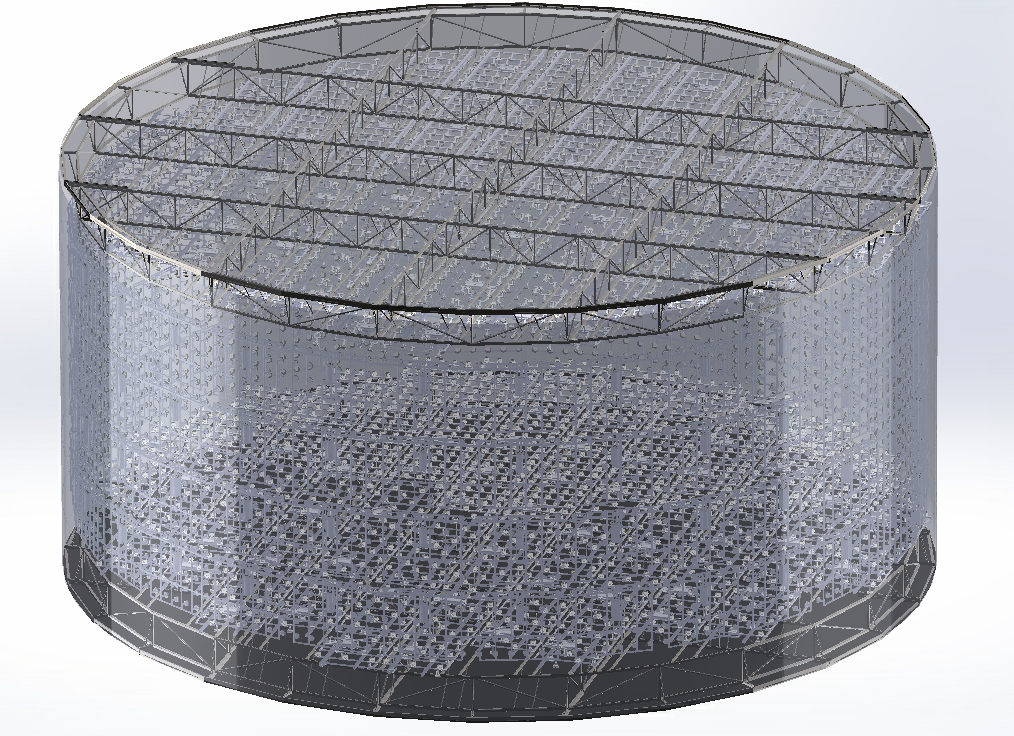
\includegraphics[width=0.8\textwidth]{diagrams/5-chips/chips_render_2.png}
    \caption[Graphical rendering of the \chipsfive detector structure.]
    {Graphical rendering of the \chipsfive detector structure.}
    \label{fig:chips_render_2}
\end{figure} %%%%%%%%%%%%%%%%%%%%%%%%%%%%%%%%%%%%%%%%%%%%%%%%%%%%%%%%%%%%%%%%%%%%%%%%%%%%%%%%%%%%%

\begin{figure} % CHIPS LOCATION IN NUMI DIAGRAM %%%%%%%%%%%%%%%%%%%%%%%%%%%%%%%%%%%%%%%%%%%%%%%%%%
    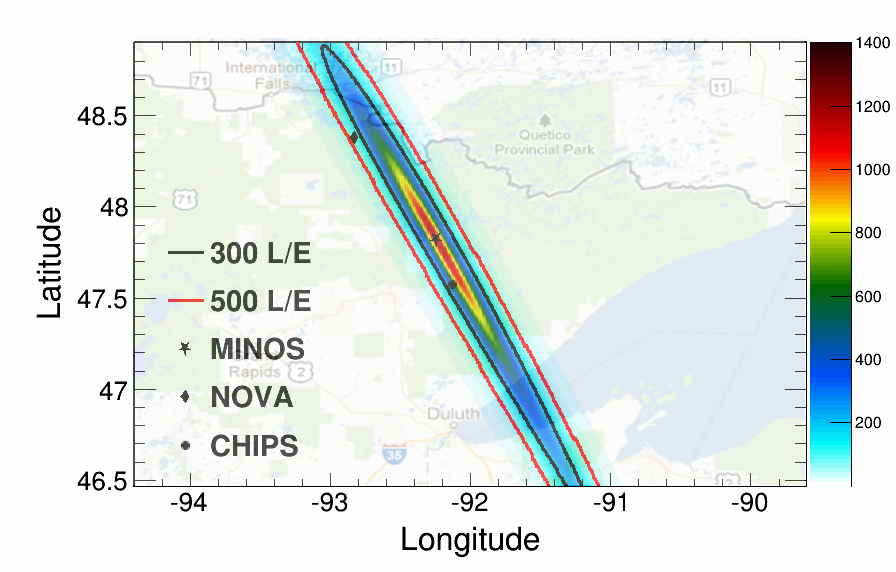
\includegraphics[width=0.8\textwidth]{diagrams/5-chips/numi_map.png}
    \caption[Map of detector locations in the \numi beam.]
    {Map of the \chips, \nova and \minos locations in the \numi beam showing the expected
        neutrino event rates, assuming no oscillations. Lines of constant L/E are shown by the
        contours. Image taken from Ref.\cite{adamson2013}.}
    \label{fig:numi_map}
\end{figure} %%%%%%%%%%%%%%%%%%%%%%%%%%%%%%%%%%%%%%%%%%%%%%%%%%%%%%%%%%%%%%%%%%%%%%%%%%%%%%%%%%%%%

\begin{figure} % NUMI BEAM DIAGRAM %%$%%%%%%%%%%%%%%%%%%%%%%%%%%%%%%%%%%%%%%%%%%%%%%%%%%%%%%%%%%%%
    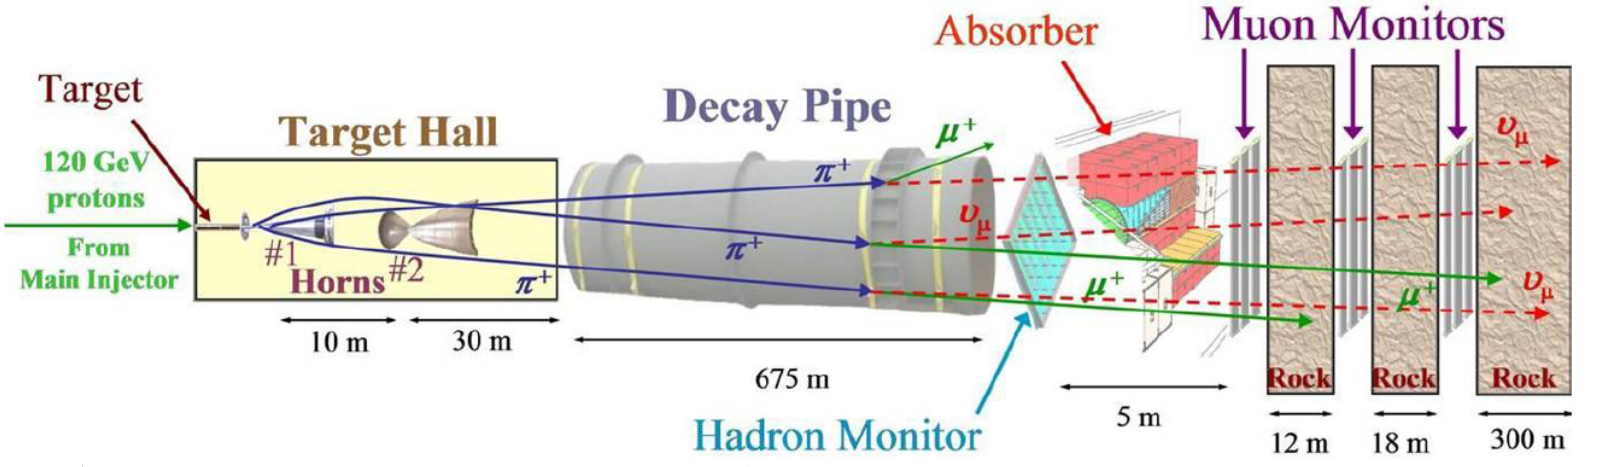
\includegraphics[width=\textwidth]{diagrams/5-chips/numi_beam.png}
    \caption[Schematic of the \numi beam.]
    {Schematic of the main components of the \numi beam (not to scale) shown with their
        dimensions. The horns control if the beam is in neutrino or anti-neutrino mode. Image
        taken from Ref.\cite{adamson2016}.}
    \label{fig:numi_beam}
\end{figure} %%%%%%%%%%%%%%%%%%%%%%%%%%%%%%%%%%%%%%%%%%%%%%%%%%%%%%%%%%%%%%%%%%%%%%%%%%%%%%%%%%%%%

\begin{figure} % OFF-AXIS FLUX DIAGRAM %%%%%%%%%%%%%%%%%%%%%%%%%%%%%%%%%%%%%%%%%%%%%%%%%%%%%%%%%%%
    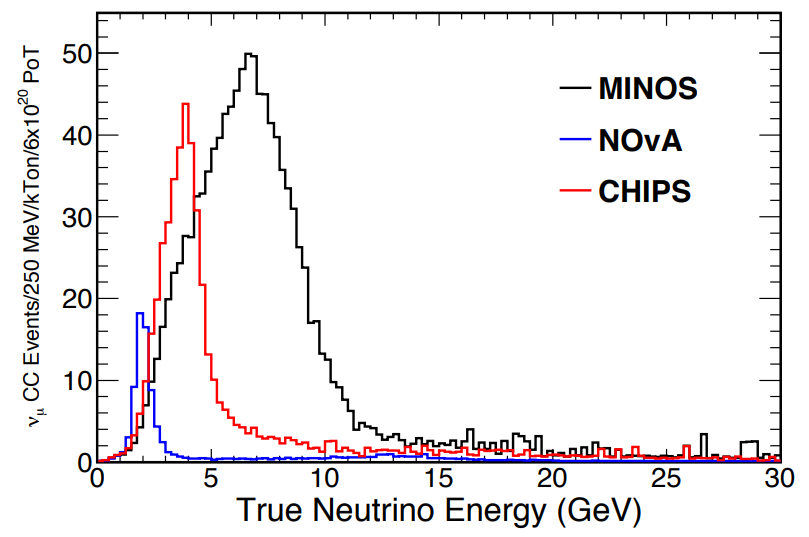
\includegraphics[width=0.8\textwidth]{diagrams/5-chips/numi_axis.png}
    \caption[Neutrino flux for different detectors in the \numi beam.]
    {Neutrino flux for different detectors in the \numi beam.
        The difference is caused by the different off-axis angles.
        Image taken from Ref.\cite{adamson2013}.}
    \label{fig:numi_axis}
\end{figure} %%%%%%%%%%%%%%%%%%%%%%%%%%%%%%%%%%%%%%%%%%%%%%%%%%%%%%%%%%%%%%%%%%%%%%%%%%%%%%%%%%%%%

\begin{figure} % CHIPS FLUX DIAGRAM %%%%%%%%%%%%%%%%%%%%%%%%%%%%%%%%%%%%%%%%%%%%%%%%%%%%%%%%%%%%%%
    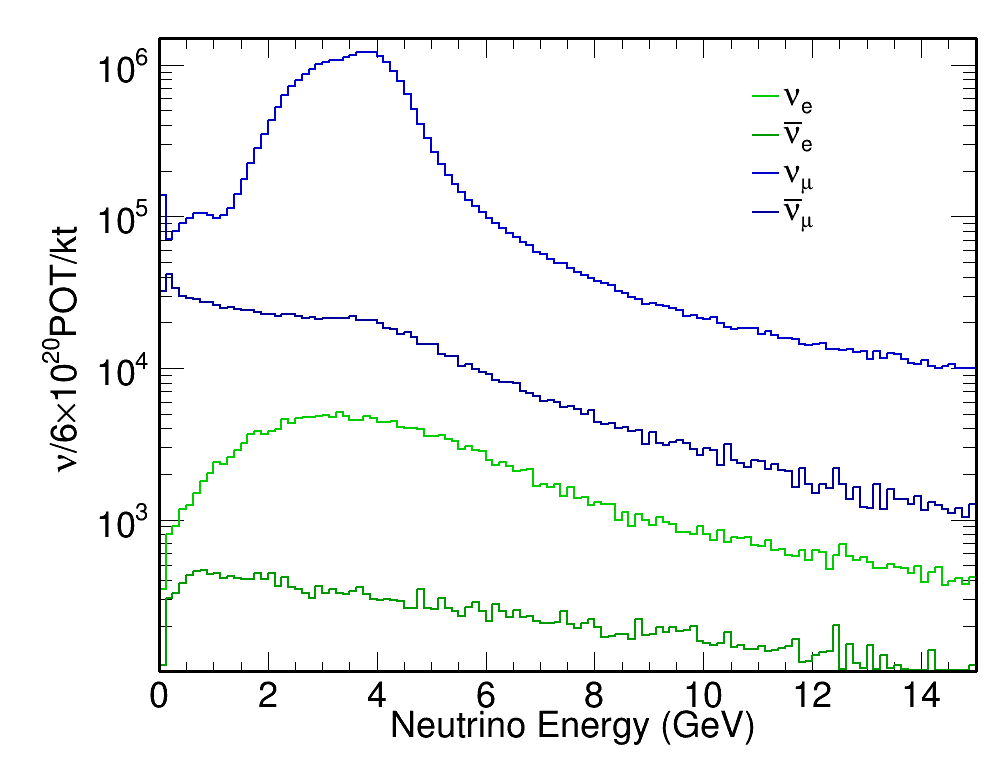
\includegraphics[width=0.8\textwidth]{diagrams/5-chips/flux.png}
    \caption[flux short]
    {}
    \label{fig:flux}
\end{figure} %%%%%%%%%%%%%%%%%%%%%%%%%%%%%%%%%%%%%%%%%%%%%%%%%%%%%%%%%%%%%%%%%%%%%%%%%%%%%%%%%%%%%

\begin{figure} % CROSS-SECTION DIAGRAM %%%%%%%%%%%%%%%%%%%%%%%%%%%%%%%%%%%%%%%%%%%%%%%%%%%%%%%%%%%
    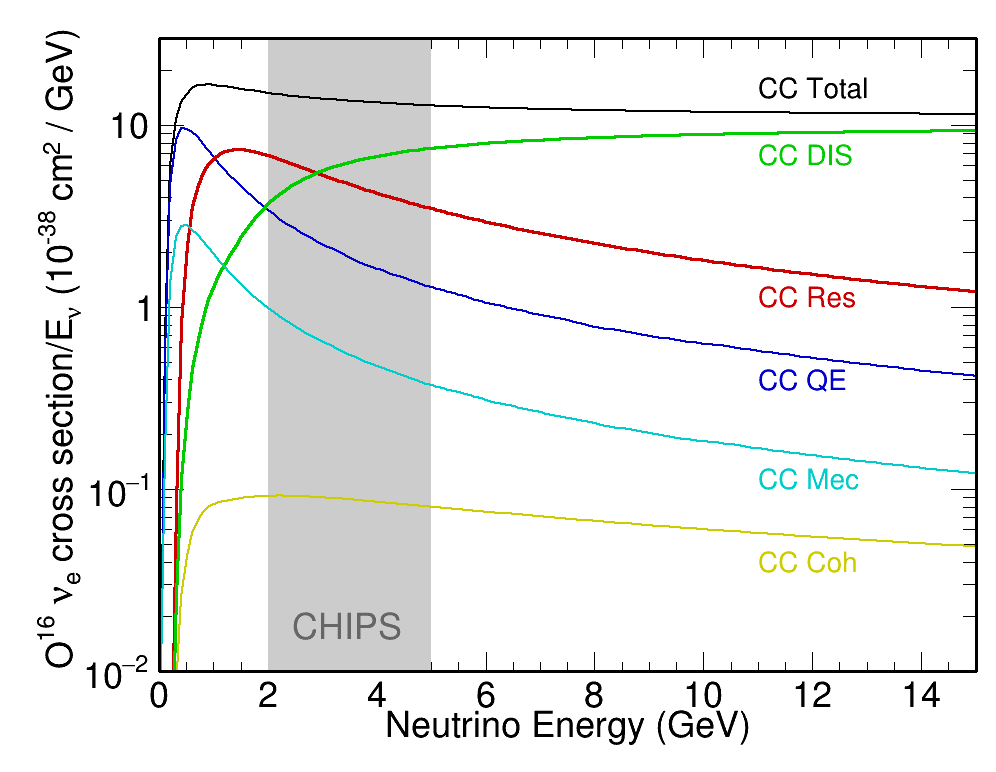
\includegraphics[width=0.8\textwidth]{diagrams/5-chips/xsec_cc_nu_e_O16.png}
    \caption[xsec cc nu e O16 short]
    {xsec cc nu e O16 long}
    \label{fig:xsec_cc_nu_e_O16}
\end{figure} %%%%%%%%%%%%%%%%%%%%%%%%%%%%%%%%%%%%%%%%%%%%%%%%%%%%%%%%%%%%%%%%%%%%%%%%%%%%%%%%%%%%%

\begin{figure} % SIMULATED EVENT DISPLAY DIAGRAM %%%%%%%%%%%%%%%%%%%%%%%%%%%%%%%%%%%%%%%%%%%%%%%%%
    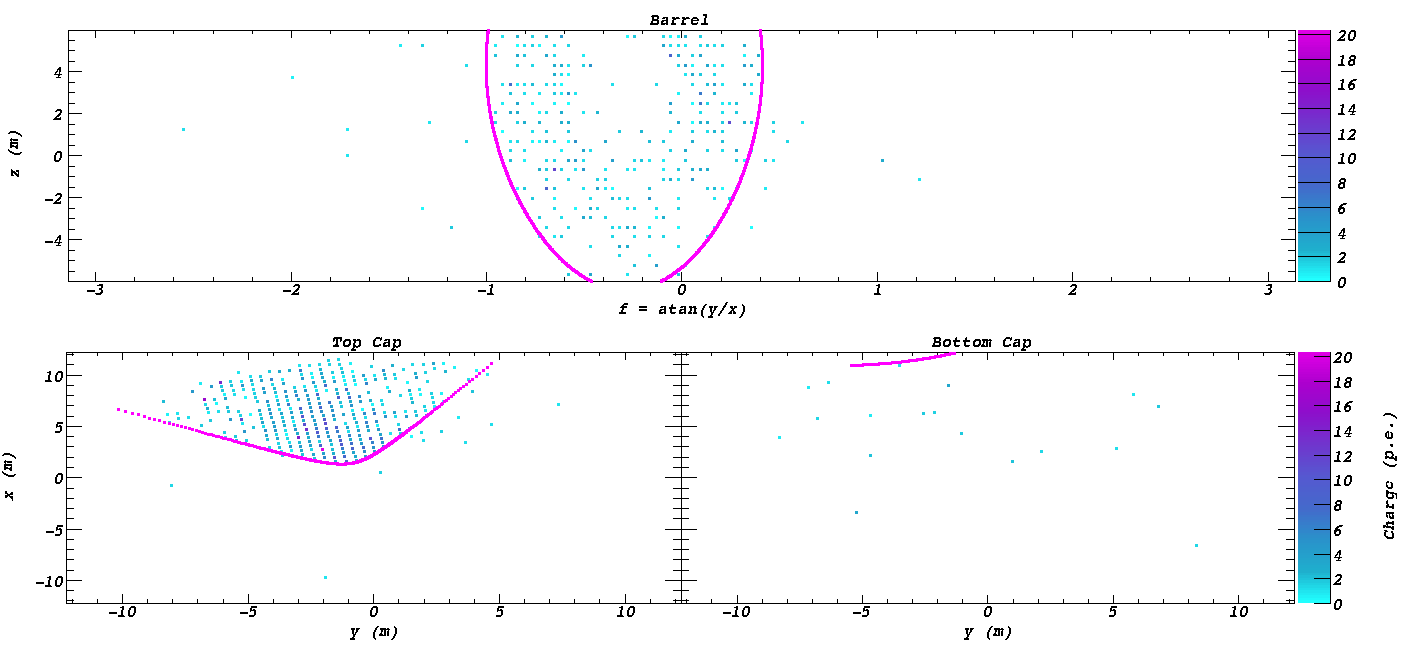
\includegraphics[width=\textwidth]{diagrams/5-chips/sim_event.png}
    \caption[sim event short]
    {$\nu_{\mu}$ CC quasi-elastic event with a single muon final state particle of energy
        1770.24 MeV}
    \label{fig:sim_event}
\end{figure} %%%%%%%%%%%%%%%%%%%%%%%%%%%%%%%%%%%%%%%%%%%%%%%%%%%%%%%%%%%%%%%%%%%%%%%%%%%%%%%%%%%%%

\begin{figure} % COSMICS AROUND DETECTOR DIAGRAM %%%%%%%%%%%%%%%%%%%%%%%%%%%%%%%%%%%%%%%%%%%%%%%%%
    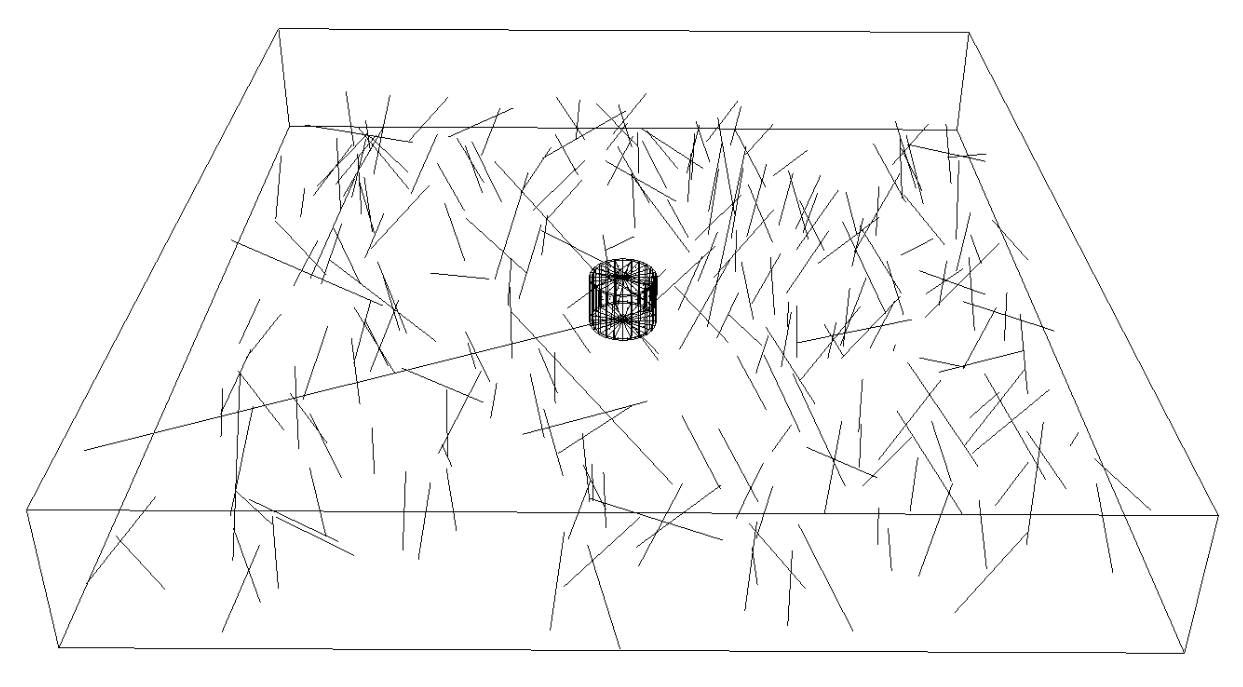
\includegraphics[width=0.8\textwidth]{diagrams/5-chips/cosmics.png}
    \caption[cosmics short]
    {cosmics long}
    \label{fig:cosmics}
\end{figure} %%%%%%%%%%%%%%%%%%%%%%%%%%%%%%%%%%%%%%%%%%%%%%%%%%%%%%%%%%%%%%%%%%%%%%%%%%%%%%%%%%%%%

DIAGRAM: POM diagram
DIAGRAM: Cosmic rate given the water overburden diagram
DIAGRAM: CHIPS fiducial volume diagram with dimensions around the sides
DIAGRAM: CHIPS expected event rate plot with and without oscillations
DIAGRAM: Cherenkov effect diagram
DIAGRAM: Floating dock diagram
DIAGRAM: Deployment diagram

- CHIPS letter of intent~\cite{adamson2013}
- CHIPS attenuation length paper~\cite{amat2017}
- CHIPS reco paper~\cite{blake2016}
- Karol prospects for CHIPS paper~\cite{lang2015}
- Andy CHIPS-M prototype construction and simulations~\cite{perch2015}
- Maciej prototype detection unit~\cite{pfutznerProto2017}
- Sensitivity Determination in the CHIPS Neutrino Detector~\cite{adde2016}
- The Numi beam big paper~\cite{adamson2016}
REF: Icecube DOM paper
REF: km3net General paper
REF: Km3net optical module paper
REF: Nemo-3 PMT paper